% Options for packages loaded elsewhere
\PassOptionsToPackage{unicode}{hyperref}
\PassOptionsToPackage{hyphens}{url}
\PassOptionsToPackage{dvipsnames,svgnames,x11names}{xcolor}
%
\documentclass[
  letterpaper,
  DIV=11,
  numbers=noendperiod]{scrartcl}

\usepackage{amsmath,amssymb}
\usepackage{iftex}
\ifPDFTeX
  \usepackage[T1]{fontenc}
  \usepackage[utf8]{inputenc}
  \usepackage{textcomp} % provide euro and other symbols
\else % if luatex or xetex
  \usepackage{unicode-math}
  \defaultfontfeatures{Scale=MatchLowercase}
  \defaultfontfeatures[\rmfamily]{Ligatures=TeX,Scale=1}
\fi
\usepackage{lmodern}
\ifPDFTeX\else  
    % xetex/luatex font selection
\fi
% Use upquote if available, for straight quotes in verbatim environments
\IfFileExists{upquote.sty}{\usepackage{upquote}}{}
\IfFileExists{microtype.sty}{% use microtype if available
  \usepackage[]{microtype}
  \UseMicrotypeSet[protrusion]{basicmath} % disable protrusion for tt fonts
}{}
\makeatletter
\@ifundefined{KOMAClassName}{% if non-KOMA class
  \IfFileExists{parskip.sty}{%
    \usepackage{parskip}
  }{% else
    \setlength{\parindent}{0pt}
    \setlength{\parskip}{6pt plus 2pt minus 1pt}}
}{% if KOMA class
  \KOMAoptions{parskip=half}}
\makeatother
\usepackage{xcolor}
\setlength{\emergencystretch}{3em} % prevent overfull lines
\setcounter{secnumdepth}{-\maxdimen} % remove section numbering
% Make \paragraph and \subparagraph free-standing
\ifx\paragraph\undefined\else
  \let\oldparagraph\paragraph
  \renewcommand{\paragraph}[1]{\oldparagraph{#1}\mbox{}}
\fi
\ifx\subparagraph\undefined\else
  \let\oldsubparagraph\subparagraph
  \renewcommand{\subparagraph}[1]{\oldsubparagraph{#1}\mbox{}}
\fi


\providecommand{\tightlist}{%
  \setlength{\itemsep}{0pt}\setlength{\parskip}{0pt}}\usepackage{longtable,booktabs,array}
\usepackage{calc} % for calculating minipage widths
% Correct order of tables after \paragraph or \subparagraph
\usepackage{etoolbox}
\makeatletter
\patchcmd\longtable{\par}{\if@noskipsec\mbox{}\fi\par}{}{}
\makeatother
% Allow footnotes in longtable head/foot
\IfFileExists{footnotehyper.sty}{\usepackage{footnotehyper}}{\usepackage{footnote}}
\makesavenoteenv{longtable}
\usepackage{graphicx}
\makeatletter
\def\maxwidth{\ifdim\Gin@nat@width>\linewidth\linewidth\else\Gin@nat@width\fi}
\def\maxheight{\ifdim\Gin@nat@height>\textheight\textheight\else\Gin@nat@height\fi}
\makeatother
% Scale images if necessary, so that they will not overflow the page
% margins by default, and it is still possible to overwrite the defaults
% using explicit options in \includegraphics[width, height, ...]{}
\setkeys{Gin}{width=\maxwidth,height=\maxheight,keepaspectratio}
% Set default figure placement to htbp
\makeatletter
\def\fps@figure{htbp}
\makeatother
% definitions for citeproc citations
\NewDocumentCommand\citeproctext{}{}
\NewDocumentCommand\citeproc{mm}{%
  \begingroup\def\citeproctext{#2}\cite{#1}\endgroup}
\makeatletter
 % allow citations to break across lines
 \let\@cite@ofmt\@firstofone
 % avoid brackets around text for \cite:
 \def\@biblabel#1{}
 \def\@cite#1#2{{#1\if@tempswa , #2\fi}}
\makeatother
\newlength{\cslhangindent}
\setlength{\cslhangindent}{1.5em}
\newlength{\csllabelwidth}
\setlength{\csllabelwidth}{3em}
\newenvironment{CSLReferences}[2] % #1 hanging-indent, #2 entry-spacing
 {\begin{list}{}{%
  \setlength{\itemindent}{0pt}
  \setlength{\leftmargin}{0pt}
  \setlength{\parsep}{0pt}
  % turn on hanging indent if param 1 is 1
  \ifodd #1
   \setlength{\leftmargin}{\cslhangindent}
   \setlength{\itemindent}{-1\cslhangindent}
  \fi
  % set entry spacing
  \setlength{\itemsep}{#2\baselineskip}}}
 {\end{list}}
\usepackage{calc}
\newcommand{\CSLBlock}[1]{\hfill\break\parbox[t]{\linewidth}{\strut\ignorespaces#1\strut}}
\newcommand{\CSLLeftMargin}[1]{\parbox[t]{\csllabelwidth}{\strut#1\strut}}
\newcommand{\CSLRightInline}[1]{\parbox[t]{\linewidth - \csllabelwidth}{\strut#1\strut}}
\newcommand{\CSLIndent}[1]{\hspace{\cslhangindent}#1}

\KOMAoption{captions}{tableheading}
\makeatletter
\@ifpackageloaded{caption}{}{\usepackage{caption}}
\AtBeginDocument{%
\ifdefined\contentsname
  \renewcommand*\contentsname{Table of contents}
\else
  \newcommand\contentsname{Table of contents}
\fi
\ifdefined\listfigurename
  \renewcommand*\listfigurename{List of Figures}
\else
  \newcommand\listfigurename{List of Figures}
\fi
\ifdefined\listtablename
  \renewcommand*\listtablename{List of Tables}
\else
  \newcommand\listtablename{List of Tables}
\fi
\ifdefined\figurename
  \renewcommand*\figurename{Figure}
\else
  \newcommand\figurename{Figure}
\fi
\ifdefined\tablename
  \renewcommand*\tablename{Table}
\else
  \newcommand\tablename{Table}
\fi
}
\@ifpackageloaded{float}{}{\usepackage{float}}
\floatstyle{ruled}
\@ifundefined{c@chapter}{\newfloat{codelisting}{h}{lop}}{\newfloat{codelisting}{h}{lop}[chapter]}
\floatname{codelisting}{Listing}
\newcommand*\listoflistings{\listof{codelisting}{List of Listings}}
\makeatother
\makeatletter
\makeatother
\makeatletter
\@ifpackageloaded{caption}{}{\usepackage{caption}}
\@ifpackageloaded{subcaption}{}{\usepackage{subcaption}}
\makeatother
\ifLuaTeX
  \usepackage{selnolig}  % disable illegal ligatures
\fi
\usepackage{bookmark}

\IfFileExists{xurl.sty}{\usepackage{xurl}}{} % add URL line breaks if available
\urlstyle{same} % disable monospaced font for URLs
\hypersetup{
  pdftitle={The Robustness of Test Statistics to Nonnormality and Specification Error in Confirmatory Factor Analysis: A Replication},
  pdfauthor={, , and },
  colorlinks=true,
  linkcolor={blue},
  filecolor={Maroon},
  citecolor={Blue},
  urlcolor={Blue},
  pdfcreator={LaTeX via pandoc}}

\title{The Robustness of Test Statistics to Nonnormality and
Specification Error in Confirmatory Factor Analysis: A
Replication\thanks{All code to generate this document is available at
github.com/jeremymiles/cwf\_replication (and this document at
jeremymiles.github.io/cwf\_replication//cwf\_replication.pdf or
jeremymiles.github.io/cwf\_replication//cwf\_replication.html) {[}Work
done while the first author was at Google{]}}}
\author{Jeremy Miles\textsuperscript{1} \and Alexander
Miles\textsuperscript{1} \and Mark Shevlin\textsuperscript{2}}
\date{2024-06-26}

\begin{document}
\maketitle
\begin{abstract}
There have been recent calls for researchers in social science
methodological research to consider replication as an This paper reports
on a replication of Curran, West, \& Finch (1996), a simulation study
that used EQS 3.0 to generate random data and analyze it in a
confirmatory factor analysis framework. We present a replication of this
simulatlion using more recently developed, open source software (the
simsem and lavaan packages in R). The results that we obtain are
substantively equivalent to the results obtained in the original paper,
but some minor discrepancies were found, and we discuss the possible
reasons. We conclude with an argument that replication of simulation
studies can be useful and informative, and thanks to the rise of open
source analysis software, websites that increase ability to share code
and improvements in computer hardware, the costs of replication are
dramatically reduced.
\end{abstract}

\textsuperscript{1} University of Southern California, Los Angeles\\
\textsuperscript{2} University of Ulster, N Ireland, UK

\section{Introduction}\label{introduction}

The replication crisis has provoked a great deal of soul searching in
many branches of science, including psychology. However, methodologists
have recently pointed out that concerns about the replication crisis
have largely passed by the methodological community (Schoenbrodt, 2023;
Strobl, 2023). A widely used tool of methodological researchers is that
of the simulation study - set up a population with a known data
generating process (DGP), take a sample of specified size from that
population, apply a statistical method and determine if the data
generating process is discovered (Carsey \& Harden, 2013). There is no
opportunity for p-hacking (in its many forms), we run the analysis and
report the results. If we run the analysis again, we get the same
results. It is perfectly replicable - no need for replication, no
replication crisis.

Lohmann, Astivia, Morris, \& Groenwold (2022) present 10 reasons that
methodological researchers should consider replicating simulation
studies.

\begin{enumerate}
\def\labelenumi{\arabic{enumi}.}
\item
  They can have a major impact. Hu \& Bentler (1999) has been cited,
  according to Google Scholar, over 113,000 times.
\item
  Simulation researchers have conflicts of interest too. Although
  conventional p-hacking would not be done in simulation studies, and
  could select the specific methods, sample sizes, etc to compare. Less
  honest researchers could even selectively choose random seeds that
  reflect their preferences.
\item
  Selective reporting. Simulation studies can include enormous numbers
  of combinations of parameters, leading to an explosion of parameters.
  Hu \& Bentler (1999) contains 8 pages of tables in the results
  section, and a further 23 pages of tables in the appendix. Most
  researchers (and readers) would prefer a more succinct paper.
\item
  Differing audiences. Simulation studies are written, reviewed, and
  read primarily by methodological researchers. A replication may be
  aimed at substantive researchers who are less interested in the
  nuances of the techniques, and more interested in knowing which
  technique is most appropriate for their problem at hand.
\item
  Code is written by (fallible) humans. The study may be designed, but
  the code needs to be written to match the design as described in the
  paper. Schonbrodt, Perugini, et al. (2018) discovered that the
  description of the study in their paper, and the accompanying code did
  not match. This is only discoverable if the code is available, which
  it frequently is not. In addition, the code runs on more software -
  even if the code that I use is accessible, the program that I run that
  code (SAS, EQS, Mplus, etc) on might not be. For example, Rigdon \&
  Ferguson Jr (1991) found that the performance of LISREL's WLS
  estimation method was not producing consistent estimation; LISREL 8.8
  made errors in the calculation of the Satorra-Bentler chi-square; AMOS
  v4.0 estimated means and intercepts, and constrained these to zero by
  default - making the null model extremely poor, and therefore
  incremental fit indices looked very, very good.
\item
  Every scenario cannot be simulated. A simulation study samples a
  specific parameter space. An analyst then tries to extrapolate to the
  particular situation that they find themselves in; a replication might
  be helpful here.
\item
  Hidden moderators. Did the initial researchers make an assumption that
  is hidden. Lohmann et al. (2022) argue that only by `\emph{getting our
  hands dirty, diving deep into the details, and actually retracing each
  step via replication}' can we uncover such threats to validity.
\item
  Replication allows us to reflect. Replicating another study is the
  best (perhaps the only) way to discover the ways in which we could
  improve our presentation
\item
  Leading by example. Methodologists argue that research should be
  clear, accessible and open. Let's show applied researchers how to do
  it.
\item
  Because we can. Replication of a simulation study is straightforward
  compared with replication of much empirical research, which ranges
  from `difficult' to `impossible and expensive'. We are in a unique
  position to be able to make contributions to the literature and
  improve the research quality of an entire field, without dealing with
  funding bodies, research ethics committees, or even needing to leave
  our desk. Given how straightforward this is, why not do it?
\end{enumerate}

To their list, we add one more. Replications are frequently software
dependent. If we find differences across software implementations, we do
not need to suggest that the authors of (complex) statistical analysis
software have made errors. Optimization algorithms improve, random
number generators differ, default convergence criteria might change.
That said, errors are sometimes discovered in

The replication crisis has made the importance of openness of code and
data more relevant, but the internet has made openness possible.
Researchers can now publish their code in Github, for (relative)
immortality. Readers of a certain age will remember the `Computer
Program Exchange' in the journal Applied Psychological Measurement, an
example of which was Whittaker, Fitzpatrick, Williams, \& Dodd (2003),
which says (in part): ``. Send a DOS-formatted 3.5-inch diskette and a
self-addressed, stamped disk mailer to \ldots{}''. I do not have a DOS
formatted diskette, I do not have a computer that can read it, and (now
I think about it) , I don't know what a disk-mailer is, and the truth
is, I can't remember the last time I used a stamp.

In this paper we present the results of a replication of a simulation
study. In 1996 the first edition of the new journal Psychological
Methods contained a paper `The Robustness of Test Statistics to
Nonnormality and Specification Error in Confirmatory Factor Analysis'
Curran et al. (1996) - we refer to this paper as CWF throughout. In the
27 years since its publication, the study has been cited 7220 times
(according to Google Scholar) and continues to be cited in contemporary
texts, e.g. Kline (2023). The authors generated data and analyzed it
using EQS version 3.0, which was released in 1989. This was (and is) a
closed source program - the current version is 7.0. The authors of CWF
did not publish their code at the time - this was not frequently done,
and was not straightforward.

We have not requested the code from the authors of CWF. We would be
unable to locate code that we (presumably) wrote around 1995 - almost 30
years from the time of writing. Even if we did have their code, we are
not aware of any researcher who has EQS version 3.0 available. The
latest version of EQS is 7.0 - we also don't have this, and when we went
to the website to determine how much it would cost, the website said
that we needed to make an enquiry. On the grounds that if we need to
ask, we can't afford it, we didn't ask. (Our total funding for this
project is \$0).

Instead of using EQS we used open source software: data were generated
using the R package simsem Pornprasertmanit, Miller, Schoemann, \&
Jorgensen (2021) and lavaan Rosseel (2012).

The aim of this paper is to, as closely as possible, replicate the
analysis carried out in the CWF paper, and determine the extent to which
the results are replicable with more recently developed software.

\section{Method}\label{method}

The CWF paper (Curran et al. (1996)) tested a series of relatively
straightforward confirmatory factor analysis model. The model had three
factors, which correlated 0.30. Each factor was indicated by three
measured variables with loadings equal to 0.7. Four model specifications
were tested: - Model 1: Correct specification. - Model 2: Two additional
cross loadings were estimated that were not in the population model. (A
misspecification of inclusion.) - Model 3: Two additional cross-loadings
of 0.35 were included in the population model that were not estimated in
the model (a misspecification of exclusion). - Model 4: Combined the
misspecification of models 2 and 3, 2 cross-loadings that existed in the
population were omitted from the fitted model, and two additional cross
loadings that were not in the population model were estimated.

Each population model was generated under three distributions:

\begin{itemize}
\tightlist
\item
  Normal distribution
\item
  Moderately non-normal (skewness = 2.0, kurtosis = 7.0)
\item
  Severely non-normal (skewness = 3.0, kurtosis = 21.0)
\end{itemize}

Four sample sizes were considered: n = 100, 200, 500, 1000.

The authors used 200 replications for each model. Given increases in
speed of computers in the 27 years since the publication of this paper,
we used 1000 replications.

Each model was estimated using maximum likelihood, and an unscaled (ML)
and Satorra-Bentler scaled (SB) chi-square statistic was calculated, and
the model was also estimated using a WLS / ADF algorithm.

Data were generated using simsem 0.5-16 and models estimated using
lavaan 0.6-17, running on R v4.3.2. (All dependencies were the latest
versions published on 2024-02-17.)

Figure~\ref{fig-pop_model_1} and Figure~\ref{fig-pop_model_2} show the
population parameters of the data generating models. The model without
cross-loadings (used for models 1 and 2) contains three latent variables
(with variance equal to 1), each of which is indicated by three measured
variables, with loadings equal to 0.7, and latent variable covariances
of 0.3. The model with cross loadings is equivalent to the previous
model, with the addition of two cross-loadings, from F1 to y7 and F3 to
y6, with loadings equal to 0.35.

\begin{figure}[H]

\centering{

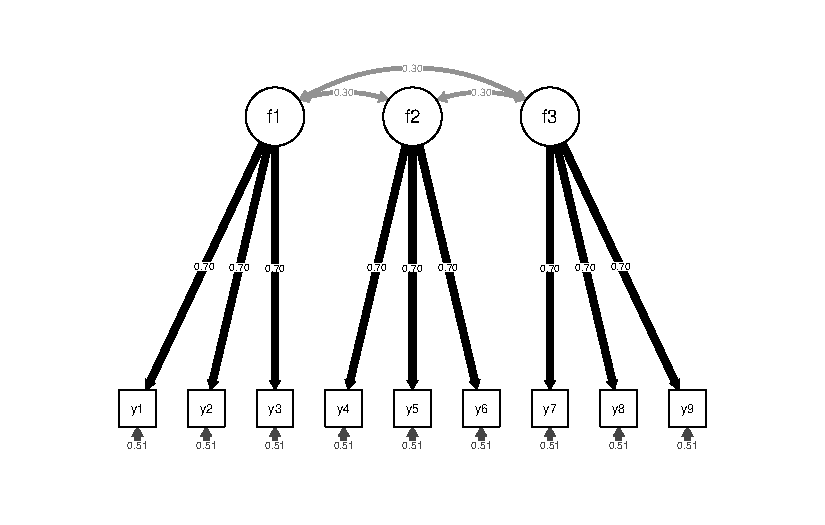
\includegraphics{cwf_replication_files/figure-pdf/fig-pop_model_1-1.pdf}

}

\caption{\label{fig-pop_model_1}Path diagram for population model
without cross loadings used.}

\end{figure}%

\begin{figure}[H]

\centering{

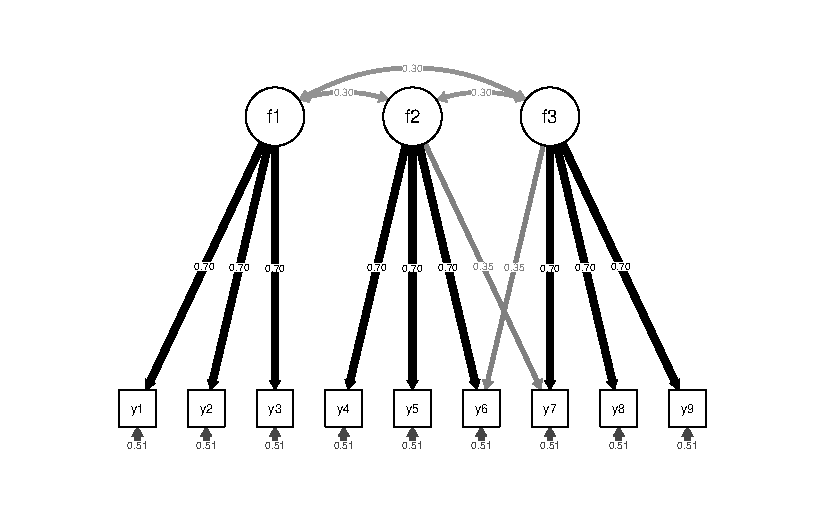
\includegraphics{cwf_replication_files/figure-pdf/fig-pop_model_2-1.pdf}

}

\caption{\label{fig-pop_model_2}Path diagram for population model with
cross loadings used.}

\end{figure}%

\section{Results}\label{results}

\subsection{Test Data Generation}\label{test-data-generation}

\subsubsection{Univariate Statistics}\label{univariate-statistics}

First, we test the data generation process to ensure that the data match
the models we believe we are testing.

To examine the deviation from normality, we generated three datasets of
size 1,000,000 for each of the three distributions (normal, moderately
non-normal, severely non-normal).

Figure~\ref{fig-dist_plot} shows the empirical distribution found from
generating all 3 datasets of interest with a sample of N = 1,000,000 and
combining all variables (so that each distribution is a sample of
9,000,000). Table~\ref{tbl-skew_stats} shows the mean, standard
deviation, median, skew and kurtosis statistics from the same dataset.

These values are a match the expected values, showing that the data
generating process we described is working as intended at least as far
as the distributions are concerned.

\begin{figure}[H]

\centering{

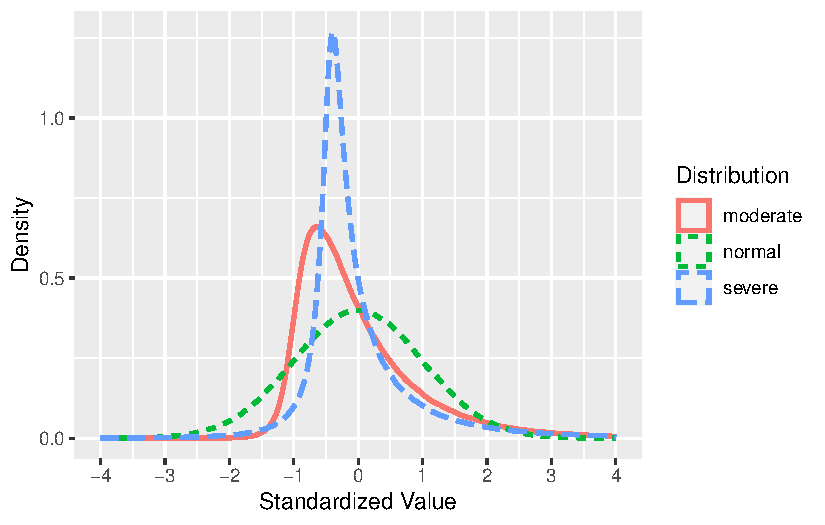
\includegraphics{cwf_replication_files/figure-pdf/fig-dist_plot-1.pdf}

}

\caption{\label{fig-dist_plot}Plots of normal, moderately non-normal and
severely non-normal empirical distributions based on N= 1,000,000.}

\end{figure}%

\begin{longtable}[]{@{}lrrrrr@{}}

\caption{\label{tbl-skew_stats}Sample statistics for empirical
distributions based on N= 1,000,000 (x 9).}

\tabularnewline

\toprule\noalign{}
& mean & sd & median & skew & kurtosis \\
\midrule\noalign{}
\endhead
\bottomrule\noalign{}
\endlastfoot
Normal & 1.03e-17 & 1 & -0.001 & 0.004 & 0.002 \\
Moderate & 1.19e-17 & 1 & -0.260 & 2.006 & 6.980 \\
Severe & -6.76e-18 & 1 & -0.252 & 3.026 & 21.371 \\

\end{longtable}

\subsubsection{Correlations}\label{correlations}

In this section we examine the empirical correlations for data with N =
1,000,000 to check that the empirical distributions match the expected
population matrices.

The correlation matrices below are calculated from each of the 6 6
distributions (2 population models, 3 distributions) with a sample size
of 1,000,000. The correlations match the values in the population
(within 0.01).

\begin{longtable}[]{@{}lrrrrrrrrr@{}}

\caption{\label{tbl-cors_data_1}Correlation Matrix for Data 1 (no cross
loadings), Normal distribution.}

\tabularnewline

\toprule\noalign{}
& y1 & y2 & y3 & y4 & y5 & y6 & y7 & y8 & y9 \\
\midrule\noalign{}
\endhead
\bottomrule\noalign{}
\endlastfoot
y1 & 1.00 & 0.49 & 0.49 & 0.15 & 0.15 & 0.15 & 0.15 & 0.15 & 0.15 \\
y2 & 0.49 & 1.00 & 0.49 & 0.15 & 0.15 & 0.15 & 0.15 & 0.15 & 0.15 \\
y3 & 0.49 & 0.49 & 1.00 & 0.15 & 0.15 & 0.15 & 0.15 & 0.15 & 0.15 \\
y4 & 0.15 & 0.15 & 0.15 & 1.00 & 0.49 & 0.49 & 0.15 & 0.15 & 0.15 \\
y5 & 0.15 & 0.15 & 0.15 & 0.49 & 1.00 & 0.49 & 0.15 & 0.15 & 0.15 \\
y6 & 0.15 & 0.15 & 0.15 & 0.49 & 0.49 & 1.00 & 0.15 & 0.15 & 0.15 \\
y7 & 0.15 & 0.15 & 0.15 & 0.15 & 0.15 & 0.15 & 1.00 & 0.49 & 0.49 \\
y8 & 0.15 & 0.15 & 0.15 & 0.15 & 0.15 & 0.15 & 0.49 & 1.00 & 0.49 \\
y9 & 0.15 & 0.15 & 0.15 & 0.15 & 0.15 & 0.15 & 0.49 & 0.49 & 1.00 \\

\end{longtable}

\begin{longtable}[]{@{}lrrrrrrrrr@{}}

\caption{\label{tbl-cors_data_2}Correlation Matrix for Data 1 (no cross
loadings), moderately non-normal distribution.}

\tabularnewline

\toprule\noalign{}
& y1 & y2 & y3 & y4 & y5 & y6 & y7 & y8 & y9 \\
\midrule\noalign{}
\endhead
\bottomrule\noalign{}
\endlastfoot
y1 & 1.00 & 0.49 & 0.49 & 0.15 & 0.15 & 0.15 & 0.15 & 0.15 & 0.15 \\
y2 & 0.49 & 1.00 & 0.49 & 0.15 & 0.15 & 0.15 & 0.15 & 0.15 & 0.15 \\
y3 & 0.49 & 0.49 & 1.00 & 0.15 & 0.15 & 0.15 & 0.15 & 0.15 & 0.15 \\
y4 & 0.15 & 0.15 & 0.15 & 1.00 & 0.49 & 0.49 & 0.15 & 0.15 & 0.15 \\
y5 & 0.15 & 0.15 & 0.15 & 0.49 & 1.00 & 0.49 & 0.15 & 0.15 & 0.15 \\
y6 & 0.15 & 0.15 & 0.15 & 0.49 & 0.49 & 1.00 & 0.15 & 0.15 & 0.15 \\
y7 & 0.15 & 0.15 & 0.15 & 0.15 & 0.15 & 0.15 & 1.00 & 0.49 & 0.49 \\
y8 & 0.15 & 0.15 & 0.15 & 0.15 & 0.15 & 0.15 & 0.49 & 1.00 & 0.49 \\
y9 & 0.15 & 0.15 & 0.15 & 0.15 & 0.15 & 0.15 & 0.49 & 0.49 & 1.00 \\

\end{longtable}

\begin{longtable}[]{@{}lrrrrrrrrr@{}}

\caption{\label{tbl-cors_data_3}Correlation Matrix for Data 1 (no cross
loadings), severely non-normal distribution.}

\tabularnewline

\toprule\noalign{}
& y1 & y2 & y3 & y4 & y5 & y6 & y7 & y8 & y9 \\
\midrule\noalign{}
\endhead
\bottomrule\noalign{}
\endlastfoot
y1 & 1.00 & 0.49 & 0.49 & 0.15 & 0.15 & 0.15 & 0.15 & 0.15 & 0.15 \\
y2 & 0.49 & 1.00 & 0.49 & 0.15 & 0.15 & 0.15 & 0.15 & 0.15 & 0.15 \\
y3 & 0.49 & 0.49 & 1.00 & 0.15 & 0.15 & 0.15 & 0.15 & 0.15 & 0.15 \\
y4 & 0.15 & 0.15 & 0.15 & 1.00 & 0.49 & 0.49 & 0.15 & 0.15 & 0.15 \\
y5 & 0.15 & 0.15 & 0.15 & 0.49 & 1.00 & 0.49 & 0.15 & 0.15 & 0.15 \\
y6 & 0.15 & 0.15 & 0.15 & 0.49 & 0.49 & 1.00 & 0.15 & 0.14 & 0.15 \\
y7 & 0.15 & 0.15 & 0.15 & 0.15 & 0.15 & 0.15 & 1.00 & 0.49 & 0.49 \\
y8 & 0.15 & 0.15 & 0.15 & 0.15 & 0.15 & 0.14 & 0.49 & 1.00 & 0.49 \\
y9 & 0.15 & 0.15 & 0.15 & 0.15 & 0.15 & 0.15 & 0.49 & 0.49 & 1.00 \\

\end{longtable}

\begin{longtable}[]{@{}lrrrrrrrrr@{}}

\caption{\label{tbl-cors_data_4}Correlation Matrix for Data 2 (cross
loadings), Normal distribution.}

\tabularnewline

\toprule\noalign{}
& y1 & y2 & y3 & y4 & y5 & y6 & y7 & y8 & y9 \\
\midrule\noalign{}
\endhead
\bottomrule\noalign{}
\endlastfoot
y1 & 1.00 & 0.49 & 0.49 & 0.15 & 0.15 & 0.19 & 0.20 & 0.15 & 0.15 \\
y2 & 0.49 & 1.00 & 0.49 & 0.15 & 0.15 & 0.19 & 0.20 & 0.15 & 0.15 \\
y3 & 0.49 & 0.49 & 1.00 & 0.15 & 0.15 & 0.20 & 0.20 & 0.15 & 0.15 \\
y4 & 0.15 & 0.15 & 0.15 & 1.00 & 0.49 & 0.50 & 0.35 & 0.15 & 0.15 \\
y5 & 0.15 & 0.15 & 0.15 & 0.49 & 1.00 & 0.50 & 0.35 & 0.15 & 0.15 \\
y6 & 0.19 & 0.19 & 0.20 & 0.50 & 0.50 & 1.00 & 0.53 & 0.35 & 0.35 \\
y7 & 0.20 & 0.20 & 0.20 & 0.35 & 0.35 & 0.53 & 1.00 & 0.50 & 0.50 \\
y8 & 0.15 & 0.15 & 0.15 & 0.15 & 0.15 & 0.35 & 0.50 & 1.00 & 0.49 \\
y9 & 0.15 & 0.15 & 0.15 & 0.15 & 0.15 & 0.35 & 0.50 & 0.49 & 1.00 \\

\end{longtable}

\begin{longtable}[]{@{}lrrrrrrrrr@{}}

\caption{\label{tbl-cors_data_5}Correlation Matrix for Data 2 (cross
loadings), moderately non-normal distribution.}

\tabularnewline

\toprule\noalign{}
& y1 & y2 & y3 & y4 & y5 & y6 & y7 & y8 & y9 \\
\midrule\noalign{}
\endhead
\bottomrule\noalign{}
\endlastfoot
y1 & 1.00 & 0.49 & 0.49 & 0.15 & 0.15 & 0.20 & 0.20 & 0.15 & 0.15 \\
y2 & 0.49 & 1.00 & 0.49 & 0.15 & 0.15 & 0.19 & 0.19 & 0.15 & 0.15 \\
y3 & 0.49 & 0.49 & 1.00 & 0.15 & 0.15 & 0.20 & 0.20 & 0.15 & 0.15 \\
y4 & 0.15 & 0.15 & 0.15 & 1.00 & 0.49 & 0.50 & 0.35 & 0.15 & 0.15 \\
y5 & 0.15 & 0.15 & 0.15 & 0.49 & 1.00 & 0.50 & 0.35 & 0.15 & 0.15 \\
y6 & 0.20 & 0.19 & 0.20 & 0.50 & 0.50 & 1.00 & 0.53 & 0.35 & 0.35 \\
y7 & 0.20 & 0.19 & 0.20 & 0.35 & 0.35 & 0.53 & 1.00 & 0.50 & 0.50 \\
y8 & 0.15 & 0.15 & 0.15 & 0.15 & 0.15 & 0.35 & 0.50 & 1.00 & 0.49 \\
y9 & 0.15 & 0.15 & 0.15 & 0.15 & 0.15 & 0.35 & 0.50 & 0.49 & 1.00 \\

\end{longtable}

\begin{longtable}[]{@{}lrrrrrrrrr@{}}

\caption{\label{tbl-cors_data_6}Correlation Matrix for Data 2 (cross
loadings), severely non-normal distribution.}

\tabularnewline

\toprule\noalign{}
& y1 & y2 & y3 & y4 & y5 & y6 & y7 & y8 & y9 \\
\midrule\noalign{}
\endhead
\bottomrule\noalign{}
\endlastfoot
y1 & 1.00 & 0.49 & 0.49 & 0.15 & 0.15 & 0.20 & 0.20 & 0.15 & 0.15 \\
y2 & 0.49 & 1.00 & 0.49 & 0.15 & 0.15 & 0.19 & 0.19 & 0.15 & 0.15 \\
y3 & 0.49 & 0.49 & 1.00 & 0.15 & 0.15 & 0.20 & 0.20 & 0.15 & 0.15 \\
y4 & 0.15 & 0.15 & 0.15 & 1.00 & 0.49 & 0.50 & 0.35 & 0.15 & 0.15 \\
y5 & 0.15 & 0.15 & 0.15 & 0.49 & 1.00 & 0.50 & 0.35 & 0.15 & 0.15 \\
y6 & 0.20 & 0.19 & 0.20 & 0.50 & 0.50 & 1.00 & 0.53 & 0.35 & 0.35 \\
y7 & 0.20 & 0.19 & 0.20 & 0.35 & 0.35 & 0.53 & 1.00 & 0.50 & 0.50 \\
y8 & 0.15 & 0.15 & 0.15 & 0.15 & 0.15 & 0.35 & 0.50 & 1.00 & 0.49 \\
y9 & 0.15 & 0.15 & 0.15 & 0.15 & 0.15 & 0.35 & 0.50 & 0.49 & 1.00 \\

\end{longtable}

\subsection{Model Fit Comparison}\label{model-fit-comparison}

In this section we compare the model fit results we obtained with those
presented in the CWF paper. In the results section we use compare the
fit statistics graphically, but full tables of results are presented in
the appendix.

\subsubsection{Model 1: Correct
Specification}\label{model-1-correct-specification}

Figure~\ref{fig-plot_chi_1} shows the mean chi-squares obtained in the
CWF paper and the current simulation. The values for the ML and SB
chi-squares are very similar. However the ADF/WLS estimates are
discrepant, and the discrepancy is larger with smaller sample sizes and
greater departure from normality. At sample sizes 500 and above the
chi-square differences are all around 1 point or less, but at smaller
sample sizes, the differences increase. In the sample size of 100, when
the distribution is normal, the difference in chi-squares is 3.6, with
moderately non-normal it is 7.2 and severely non-normal the difference
increases to 15.6. the

\begin{figure}[H]

\centering{

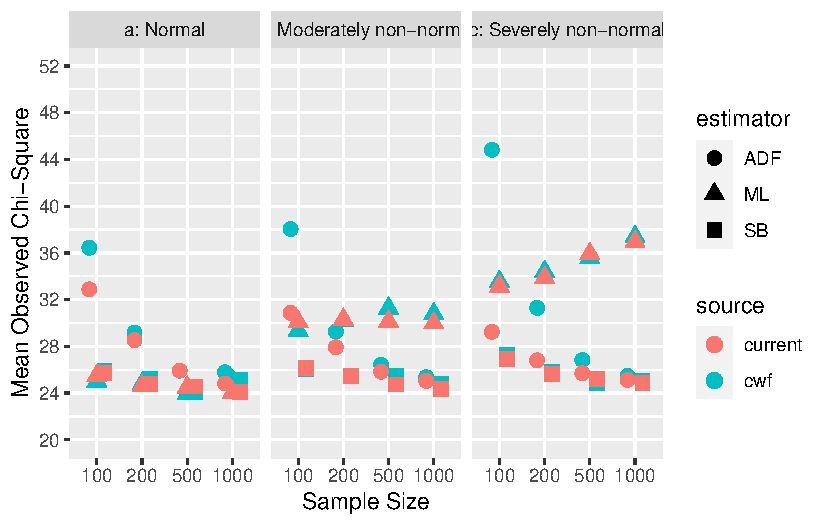
\includegraphics{cwf_replication_files/figure-pdf/fig-plot_chi_1-1.pdf}

}

\caption{\label{fig-plot_chi_1}Model 1: Correct Specification. Mean
chi-square values obtained from three estimators in CWF paper and
current simulation}

\end{figure}%

The story is repeated when we consider rejection rates, shown in
Figure~\ref{fig-plot_rejects_1}. Proportion of models were p \textless{}
0.05 is very similar for ML and SB, but there are quite dramatic
differences in rejection rates for ADF/WLS at smaller samples, with CWF
finding higher rejection rates with small samples, and this difference
increases as the degree of non-normality increases.

\begin{figure}[H]

\centering{

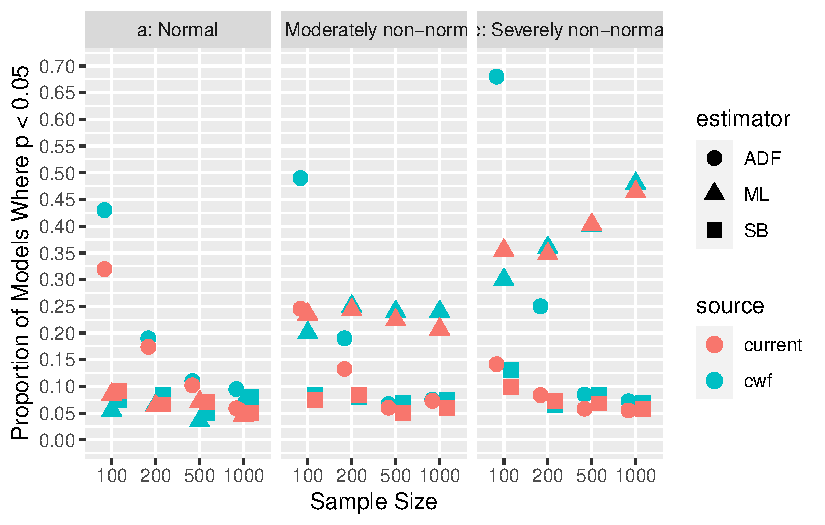
\includegraphics{cwf_replication_files/figure-pdf/fig-plot_rejects_1-1.pdf}

}

\caption{\label{fig-plot_rejects_1}Model 1: Correct Specification.
Proportion of models where p \textless{} 0.05 obtained from three
estimators in CWF paper and current simulation}

\end{figure}%

\subsubsection{Model 2: Inclusion
Misspecification}\label{model-2-inclusion-misspecification}

Figure~\ref{fig-plot_chi_2} shows the mean chi-squares obtained in the
CWF paper and the current simulation for model 2 (which had a
misspecification of inclusion). These results are substantively
equivalent to those for model 1: SB and ML are similar, ADF/WLS is
larger in CWF, and the differences are larger with smaller sample sizes
and greater deviation from normality.

\begin{figure}[H]

\centering{

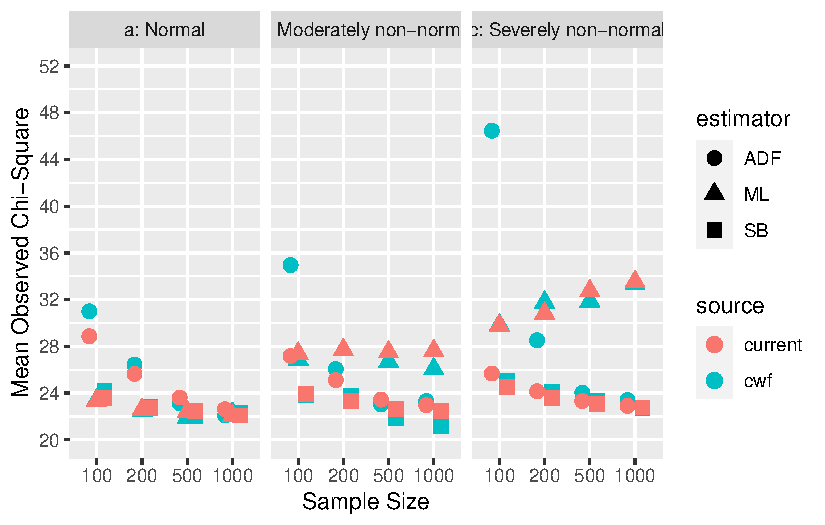
\includegraphics{cwf_replication_files/figure-pdf/fig-plot_chi_2-1.pdf}

}

\caption{\label{fig-plot_chi_2}Model 1: Correct Specification. Mean
chi-square values obtained from three estimators in CWF paper and
current simulation}

\end{figure}%

Differences in rejection rates for model 2 reflect those of model 1, as
shown in Figure~\ref{fig-plot_rejects_2}. Rejection rates were found to
be higher in the CWF paper than in the current simulation, for small
samples and deviation from normality.

\begin{figure}[H]

\centering{

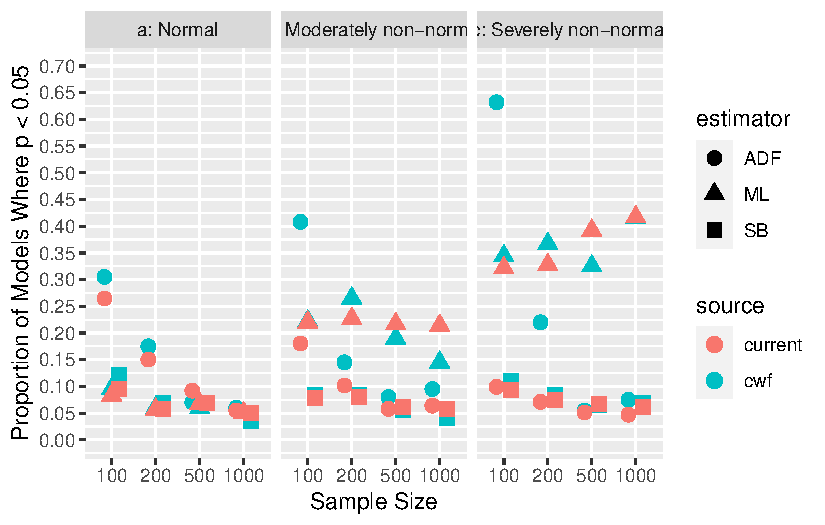
\includegraphics{cwf_replication_files/figure-pdf/fig-plot_rejects_2-1.pdf}

}

\caption{\label{fig-plot_rejects_2}Model 2: Correct Specification.
Proportion of models where p \textless{} 0.05 obtained from three
estimators in CWF paper and current simulation}

\end{figure}%

\subsubsection{Model 3: Exclusion
Misspecification}\label{model-3-exclusion-misspecification}

Figure~\ref{fig-plot_chi_3} shows the mean chi-squares obtained in the
CWF paper and the current simulation for model 3 (which had a
misspecification of exclusion). Here we see larger differences between
the current simulation and those presented in CWF. The CWF paper has
larger average chi-squares than we found, but this difference is
consistent for all three estimators, but larger for the ADF/WLS
estimator than ML and SB. Unlike the previous models, the discrepancies
are also larger in larger sample sizes.

\begin{figure}[H]

\centering{

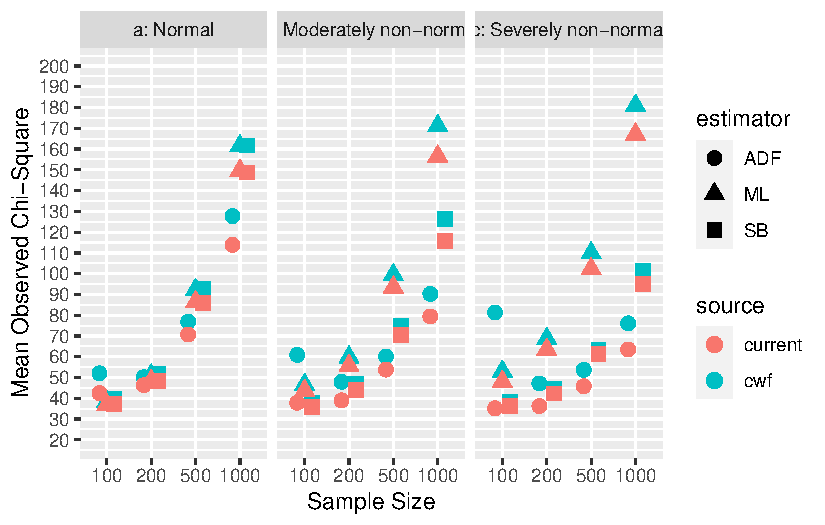
\includegraphics{cwf_replication_files/figure-pdf/fig-plot_chi_3-1.pdf}

}

\caption{\label{fig-plot_chi_3}Model 3: Incorrect Specification
Exclusion. Mean chi-square values obtained from three estimators in CWF
paper and current simulation}

\end{figure}%

The differences in rejection rates for model 3 are consistent with the
differences chi-square statistics, and can be seen in
Figure~\ref{fig-plot_rejects_3}. At larger sample sizes the rejection
rates essentially asymptote at 1, hence differences are not seen, but at
smaller sample sizes the discrepancies between the models is large.

\begin{figure}[H]

\centering{

\captionsetup{labelsep=none}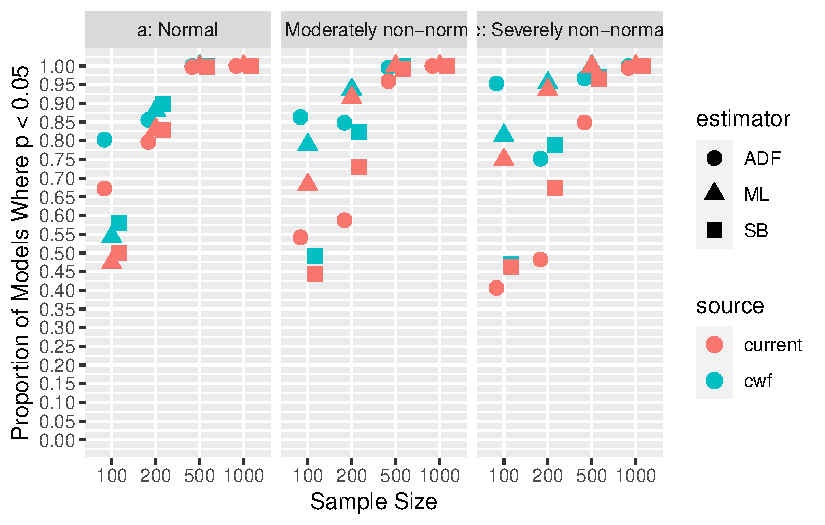
\includegraphics{cwf_replication_files/figure-pdf/fig-plot_rejects_3-1.pdf}

}

\caption{\label{fig-plot_rejects_3}}

\end{figure}%

\subsubsection{Model 4: Exclusion and Inclusion
Misspecification}\label{model-4-exclusion-and-inclusion-misspecification}

Figure~\ref{fig-plot_chi_3} shows the mean chi-squares obtained in the
CWF paper and the current simulation for model 3 (which had a
misspecification of exclusion). Here we see larger differences between
the current simulation and those presented in CWF. The CWF paper has
larger average chi-squares than we found, but this difference is
consistent for all three estimators, but larger for the ADF/WLS
estimator than ML and SB. Unlike the previous models, the discrepancies
are also larger in larger sample sizes.

\begin{figure}[H]

\centering{

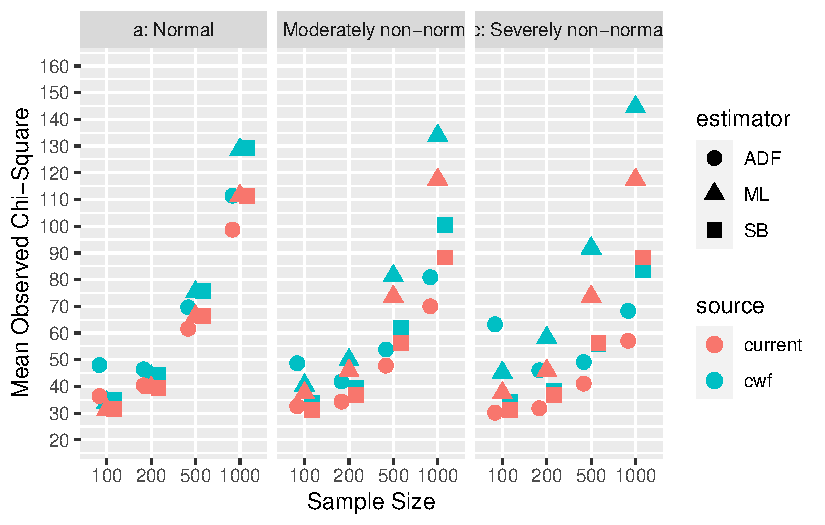
\includegraphics{cwf_replication_files/figure-pdf/fig-plot_chi_4-1.pdf}

}

\caption{\label{fig-plot_chi_4}Model 4: Incorrect Specification -
Exclusion + Inclusion. Mean chi-square values obtained from three
estimators in CWF paper and current simulation}

\end{figure}%

The differences in rejection rates for model 3 are consistent with the
differences chi-square statistics, and can be seen in
Figure~\ref{fig-plot_rejects_3}. At larger sample sizes the rejection
rates essentially asymptote at 1, hence differences are not seen, but at
smaller sample sizes the discrepancies between the models is large.

\begin{figure}[H]

\centering{

\captionsetup{labelsep=none}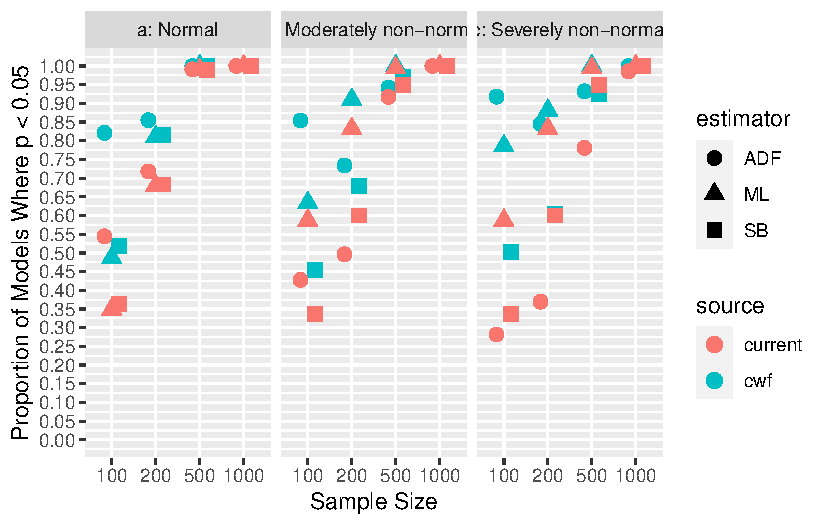
\includegraphics{cwf_replication_files/figure-pdf/fig-plot_rejects_4-1.pdf}

}

\caption{\label{fig-plot_rejects_4}}

\end{figure}%

\subsection{Expected Values of
Chi-Square}\label{expected-values-of-chi-square}

The Satorra-Saris (Satorra \& Saris, 1985) method can be used to
calculate the expected value of chi-square, given ML estimation and
normally distributed data. For models 1 and 2 this value is trivial to
calculate, as the models are correctly specified (or when they are
incorrect, the error is one of inclusion) hence the expected chi-square
values are equal to the degrees of freedom in the model. For models 3
and 4 we calculate the expected values of chi-square using the
Satorra-Saris method (which is described in more detail in CWF).

The expected values that we calculate are consistently lower than the
expected values calculated by CWF. It appears that for each simulation
(this one, and CWF), the expected values of chi-square are a closer
match to the mean observed value. For example, for Model 3, sample size
100, the current study's calculated expected value of chi-square is
36.45 and the mean observed value is 36.84; for CWF, the expected value
is 37.62 and the observed is 38.45. For model 4, sample size 1000,
current study expected: 110.44, observed 111.37, for CWF the values are
128.20 and 128.71.

\begin{longtable}[]{@{}
  >{\raggedleft\arraybackslash}p{(\columnwidth - 8\tabcolsep) * \real{0.0649}}
  >{\raggedleft\arraybackslash}p{(\columnwidth - 8\tabcolsep) * \real{0.2987}}
  >{\raggedleft\arraybackslash}p{(\columnwidth - 8\tabcolsep) * \real{0.1688}}
  >{\raggedleft\arraybackslash}p{(\columnwidth - 8\tabcolsep) * \real{0.2987}}
  >{\raggedleft\arraybackslash}p{(\columnwidth - 8\tabcolsep) * \real{0.1688}}@{}}

\caption{\label{tbl-expected_chis}Expected values of chi-square for
models 3 and 4 in current study and CWF}

\tabularnewline

\toprule\noalign{}
\begin{minipage}[b]{\linewidth}\raggedleft
n
\end{minipage} & \begin{minipage}[b]{\linewidth}\raggedleft
Model 3: Current Study
\end{minipage} & \begin{minipage}[b]{\linewidth}\raggedleft
Model 3: CWF
\end{minipage} & \begin{minipage}[b]{\linewidth}\raggedleft
Model 4: Current Study
\end{minipage} & \begin{minipage}[b]{\linewidth}\raggedleft
Model 4: CWF
\end{minipage} \\
\midrule\noalign{}
\endhead
\bottomrule\noalign{}
\endlastfoot
100 & 36.45 & 37.62 & 30.84 & 32.52 \\
200 & 48.91 & 51.38 & 39.69 & 43.14 \\
500 & 86.27 & 92.66 & 66.22 & 75.04 \\
1000 & 148.54 & 161.35 & 110.44 & 128.20 \\

\end{longtable}

One possible explanation for this discrepancy is that the error
variances were misreported in Figure 1 of CWF. Figure 1 of CWF shows
that each of the measured variables has a residual variance of 0.51 in
both the model with and without the cross loadings. If this is the case,
when the cross loading is added to the model, the variance of the item
must increase.

The CFA model presented in Figure 1 of the paper suggests that in the
population models without cross loadings, the variance of all items is
1.00, but in the models with cross loadings, the variance of items 6 and
7 increases to 1.269, while all of the other items have variances equal
to 1.

To test this hypothesis, we modified the population model so that the
residual variances of items 6 and 7 were not 0.51 in the population
model, but were 0.25. This change meant that the implied variances of
all of the items was 1.00. The path diagram, drawn from the model, is
shown in Figure~\ref{fig-pop_model_new}, and the calculated expected
values of chi-square from the modified model alongside the values
presented in CWF are shown in Table~\ref{tbl-expected_chis_modified}.

\begin{figure}[H]

\centering{

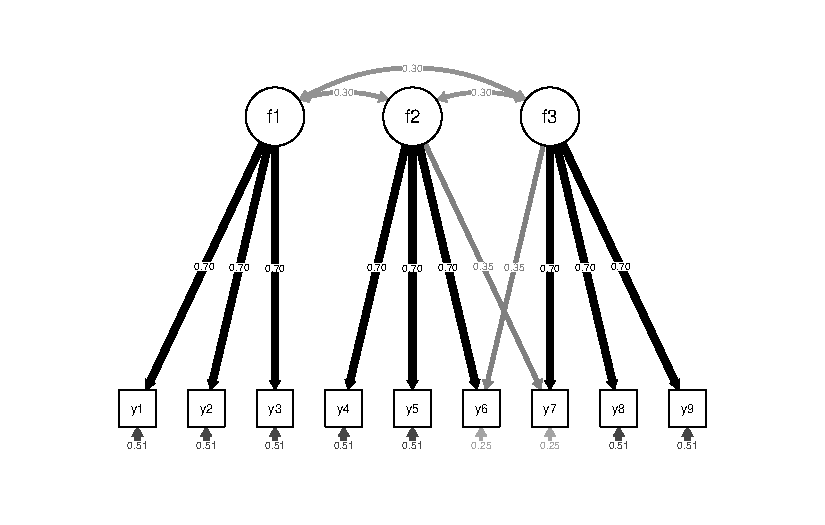
\includegraphics{cwf_replication_files/figure-pdf/fig-pop_model_new-1.pdf}

}

\caption{\label{fig-pop_model_new}Path diagram for population model with
cross loadings and modified residual variance}

\end{figure}%

\begin{longtable}[]{@{}
  >{\raggedleft\arraybackslash}p{(\columnwidth - 8\tabcolsep) * \real{0.0746}}
  >{\raggedleft\arraybackslash}p{(\columnwidth - 8\tabcolsep) * \real{0.2687}}
  >{\raggedleft\arraybackslash}p{(\columnwidth - 8\tabcolsep) * \real{0.1940}}
  >{\raggedleft\arraybackslash}p{(\columnwidth - 8\tabcolsep) * \real{0.2687}}
  >{\raggedleft\arraybackslash}p{(\columnwidth - 8\tabcolsep) * \real{0.1940}}@{}}

\caption{\label{tbl-expected_chis_modified}Expected values of chi-square
for models 3 and 4 in current study and CWF}

\tabularnewline

\toprule\noalign{}
\begin{minipage}[b]{\linewidth}\raggedleft
n
\end{minipage} & \begin{minipage}[b]{\linewidth}\raggedleft
Model 3: Modified
\end{minipage} & \begin{minipage}[b]{\linewidth}\raggedleft
Model 3: CWF
\end{minipage} & \begin{minipage}[b]{\linewidth}\raggedleft
Model 4: Modified
\end{minipage} & \begin{minipage}[b]{\linewidth}\raggedleft
Model 4: CWF
\end{minipage} \\
\midrule\noalign{}
\endhead
\bottomrule\noalign{}
\endlastfoot
100 & 37.97 & 37.62 & 32.62 & 32.52 \\
200 & 51.95 & 51.38 & 43.24 & 43.14 \\
500 & 93.87 & 92.66 & 75.09 & 75.04 \\
1000 & 163.73 & 161.35 & 128.19 & 128.20 \\

\end{longtable}

We count a simulation as a proper solution the lavaan::cfa() function
reports that the model converged, and if the solution is proper -
i.e.~all residual variances are positive (no Heywood cases). The CWF
paper reports that 90\% of the replications were proper for ML and 83\%
were proper for ADF.

Table~\ref{tbl-convergence_percs} shows the percentage of models for
each cell of the simulation that converged on a proper solution.
Unsurprisingly, convergence as associated with sample size (smaller
samples led to less convergence) estimator (ADF was less likely to
converge than ML) and degree of departure from non-normality. The
severely non-normal, ADF estimator with N = 100 converged in only 57.5\%
of simulations.

Table~\ref{tbl-convergence_percs_summary} shows the mean convergence for
each estimator. The convergence rates achieved in this simulation were
higher than those reported by CWF.

\begin{longtable}[]{@{}rlrrr@{}}

\caption{\label{tbl-convergence_percs}Percentage of models in each cell
that converged}

\tabularnewline

\toprule\noalign{}
model & distribution & size & ML & ADF \\
\midrule\noalign{}
\endhead
\bottomrule\noalign{}
\endlastfoot
1 & a: Normal & 100 & 99.9 & 94.2 \\
1 & b: Moderately non-normal & 100 & 98.7 & 87.2 \\
1 & c: Severely non-normal & 100 & 93.6 & 79.1 \\
2 & a: Normal & 100 & 99.6 & 93.7 \\
2 & b: Moderately non-normal & 100 & 96.8 & 86.0 \\
2 & c: Severely non-normal & 100 & 89.5 & 76.6 \\
3 & a: Normal & 100 & 94.7 & 87.2 \\
3 & b: Moderately non-normal & 100 & 91.3 & 78.3 \\
3 & c: Severely non-normal & 100 & 85.4 & 63.0 \\
4 & a: Normal & 100 & 94.5 & 81.4 \\
4 & b: Moderately non-normal & 100 & 86.7 & 73.4 \\
4 & c: Severely non-normal & 100 & 86.7 & 57.5 \\
1 & a: Normal & 200 & 100.0 & 100.0 \\
1 & b: Moderately non-normal & 200 & 100.0 & 99.6 \\
1 & c: Severely non-normal & 200 & 99.8 & 96.8 \\
2 & a: Normal & 200 & 100.0 & 99.8 \\
2 & b: Moderately non-normal & 200 & 100.0 & 99.4 \\
2 & c: Severely non-normal & 200 & 99.8 & 95.6 \\
3 & a: Normal & 200 & 99.8 & 99.3 \\
3 & b: Moderately non-normal & 200 & 99.3 & 93.3 \\
3 & c: Severely non-normal & 200 & 96.9 & 82.7 \\
4 & a: Normal & 200 & 99.9 & 98.2 \\
4 & b: Moderately non-normal & 200 & 98.3 & 91.3 \\
4 & c: Severely non-normal & 200 & 98.3 & 79.6 \\
1 & a: Normal & 500 & 100.0 & 100.0 \\
1 & b: Moderately non-normal & 500 & 100.0 & 100.0 \\
1 & c: Severely non-normal & 500 & 100.0 & 99.8 \\
2 & a: Normal & 500 & 100.0 & 100.0 \\
2 & b: Moderately non-normal & 500 & 100.0 & 100.0 \\
2 & c: Severely non-normal & 500 & 100.0 & 99.7 \\
3 & a: Normal & 500 & 100.0 & 100.0 \\
3 & b: Moderately non-normal & 500 & 100.0 & 98.6 \\
3 & c: Severely non-normal & 500 & 99.8 & 91.4 \\
4 & a: Normal & 500 & 100.0 & 100.0 \\
4 & b: Moderately non-normal & 500 & 100.0 & 97.8 \\
4 & c: Severely non-normal & 500 & 100.0 & 93.6 \\
1 & a: Normal & 1000 & 100.0 & 100.0 \\
1 & b: Moderately non-normal & 1000 & 100.0 & 100.0 \\
1 & c: Severely non-normal & 1000 & 100.0 & 99.9 \\
2 & a: Normal & 1000 & 100.0 & 100.0 \\
2 & b: Moderately non-normal & 1000 & 100.0 & 100.0 \\
2 & c: Severely non-normal & 1000 & 100.0 & 99.9 \\
3 & a: Normal & 1000 & 100.0 & 100.0 \\
3 & b: Moderately non-normal & 1000 & 100.0 & 99.8 \\
3 & c: Severely non-normal & 1000 & 100.0 & 96.8 \\
4 & a: Normal & 1000 & 100.0 & 100.0 \\
4 & b: Moderately non-normal & 1000 & 100.0 & 99.9 \\
4 & c: Severely non-normal & 1000 & 100.0 & 97.4 \\

\end{longtable}

\begin{longtable}[]{@{}lr@{}}

\caption{\label{tbl-convergence_percs_summary}Percentage of models using
each estimator that converged}

\tabularnewline

\toprule\noalign{}
& Percent Proper \\
\midrule\noalign{}
\endhead
\bottomrule\noalign{}
\endlastfoot
ML & 98.1 \\
ADF & 93.1 \\

\end{longtable}

\section{Discussion}\label{discussion}

In this paper we replicated, as precisely as possible, a simulation
study originally presented by Curran et al. (1996). Where the data
generation and analysis was done using EQS 3.0, we used the R packages
simsem and lavaan.

Overall, our results were substantively similar and the conclusions
about the appropriateness of the different estimators would not have
been altered by the differences between our results.

One difference that stands out is the performance of the ADF/WLS
estimator in smaller samples. The simulations run in lavaan have lower
chi-squares and lower rejection rates than the simulations run in the
CWF paper. These differences increase as the distributions deviate
further from normality. With model 1 (correct model), normal
distribution and N = 100, the mean observed ADF/WLS chi-square is 32.9
in the current simulation, and 36.4 in the CWF paper, but for the
severely non-normal data, the values are 29.2 and 44.8. However, with a
sample size of 1000, the values for normal are 24.8 (current) and 25.8
(CWF); for severely non-normal 25.1 (current) and 25.5 (CWF). The ML and
SB estimators of these models were very similar.

It is possible that difference in convergence rates might have resulted
in these differences. The lavaan models converged at a much higher rate
than the EQS models reported in CWF. EQS uses a Gauss-Newton method for
optimization, lavaan (by default) uses a quasi-Newton approach. If the
model fails to converge in lavaan, the program will attempt to refit, up
to 4 times, with different starting values and scaling settings
(Rosseel, personal communication). If the ADF/WLS models with higher
chi-square statistics failed to converge in lavaan, but did converge in
EQS, the resulting sample bias could skew these statistics. Altering the
tolerance for convergence might reduce or eliminate these differences.

A second difference between the results was also intriguing. The
chi-square values obtained in the original paper were consistently
higher than the results that we obtained, for almost all estimators at
all sample sizes - even for the correctly specified models. When we
compared the expected chi-squares, which are calculation based, not
simulation based, these differences remained - the expected chi-square
values of Curran, et al, were similar to the obtained chi-square values
that they found via simulation. The expected chi-square values that we
calculated were more similar to the obtained chi-square values that we
found via simulation.

We believe that this difference may be due to an inconsistency in the
presentation in a figure in the table. Residual variances were possibly
erroneously reported as being equal in all models, where in models with
cross-loadings these residual variances may have been reduced. The
change in residual variance is easy to overlook as this is not a part of
the model that one is generally particularly interested in, and we
rarely make or test hypotheses about the estimates of residual
variances.

However, this exercise leads to some more general conclusions, not
specifically regarding this paper. Presenting a simulation study in
sufficient detail in a conventional journal article that it can be
replicated precisely is challenging - if authors do not share the code,
it can be difficult for others to replicate and thereby confirm (or at
least support) the results. Sharing code was not straightforward in
1996, but now we have websites like Github, which support sharing of
code, and osf.io, which support sharing of code and other information.

In this paper we have used the semPlot package (Epskamp, 2022) to draw
path diagrams based on the models that we fitted. Although we believe
that we can draw path diagrams that are more esthetically pleasing using
other programs, the use of semPlot (or similar software) which takes the
fitted model as input and draws output ensures that the path diagram
matches the models.

The cost in both time and hardware of running simulations has been
dramatically reduced, thanks to Moore's law. The original simulation was
run on a 386 computer with a 20MB hard drive. Curran (personal
communication) says that the simulations took `days and days' and had
several tweaks to try to speed them up. The simulations in the current
paper were run on a 3 year old consumer PC that is primarily used to
play Civilization and online Chess. We ran five times more simulations
(1000 vs 200), and the whole analysis took approximately an hour to run,
Rstudio saves a cache file that is 80MB (or 4x more than the computer
these were originally run on), and it requires about 15GB of RAM. We
could write more efficient code and reduce these dramatically (an
earlier version used around 50GB of RAM and saved an 8 GB file), but our
attention spans are limited, and hardware is cheap (essentially free, we
can continue to play chess while the simulations run). If our time were
even more valuable, we could rent a computer from a cloud provider, and
a cost of around \$6 per hour, increase the speed by a factor of
approximately 15. Our more serious point is that the hurdles that must
be overcome to do this work are dramatically reduced, and the benefits
are potentially high.

Fairchild, Yin, Baraldi, Astivia, \& Shi (2024) also replicated the
Curran, et al, paper in a thorough and thoughtful investigation. They
also found that the results were generally consistent but with some
differences. Specifically, they focused on the data generation method
for the non-normal distributions - which is not something that we
considered in our investigation. They found that different data
generation methods for non-normal data led to different results. We
cannot conclude that the differences that we found in this research are
not due to data generation differences.

Finally, the experience of carrying out this work has shown that, for us
at least, it is very difficult to fully evaluate a simulation study by
reading it, and not replicating it. The authors of CWF acknowledge both
Peter Bentler and Douglas Bonett - SEM practitioners and researchers
that one would generally defer to, but it appears that neither of these
researchers noted the omission of the change in the residual variances.
In addition, if any of the 7000+ authors who have cited this paper have
made this connection, it has not been brought to our attention.

\section{Acknowledgments}\label{acknowledgments}

We thank Preston Botter, Patrick Curran and Yves Rosseel for discussion
and comments on different aspects of this paper. (And for catching our
worst errors.)

\section*{References}\label{references}
\addcontentsline{toc}{section}{References}

\phantomsection\label{refs}
\begin{CSLReferences}{1}{0}
\bibitem[\citeproctext]{ref-carsey2013monte}
Carsey, T. M., \& Harden, J. J. (2013). \emph{Monte carlo simulation and
resampling methods for social science}. Sage Publications.

\bibitem[\citeproctext]{ref-curran1996robustness}
Curran, P. J., West, S. G., \& Finch, J. F. (1996). The robustness of
test statistics to nonnormality and specification error in confirmatory
factor analysis. \emph{Psychological methods}, \emph{1}(1), 16.

\bibitem[\citeproctext]{ref-EpskampSemPlot}
Epskamp, S. (2022). \emph{semPlot: Path diagrams and visual analysis of
various SEM packages' output}. Retrieved from
\url{https://CRAN.R-project.org/package=semPlot}

\bibitem[\citeproctext]{ref-fairchild2024many}
Fairchild, A. J., Yin, Y., Baraldi, A. N., Astivia, O. L. O., \& Shi, D.
(2024). Many nonnormalities, one simulation: Do different data
generation algorithms affect study results? \emph{Behavior Research
Methods}, 1--21. Springer.

\bibitem[\citeproctext]{ref-hu1999cutoff}
Hu, L., \& Bentler, P. M. (1999). Cutoff criteria for fit indexes in
covariance structure analysis: Conventional criteria versus new
alternatives. \emph{Structural equation modeling: a multidisciplinary
journal}, \emph{6}(1), 1--55.

\bibitem[\citeproctext]{ref-kline2023principles}
Kline, R. B. (2023). \emph{Principles and practice of structural
equation modeling}. Guilford publications.

\bibitem[\citeproctext]{ref-lohmann2022s}
Lohmann, A., Astivia, O. L., Morris, T. P., \& Groenwold, R. H. (2022).
It's time! Ten reasons to start replicating simulation studies.
\emph{Frontiers in Epidemiology}, \emph{2}, 973470.

\bibitem[\citeproctext]{ref-simsem}
Pornprasertmanit, S., Miller, P., Schoemann, A., \& Jorgensen, T. D.
(2021). \emph{Simsem: SIMulated structural equation modeling}. Retrieved
from \url{https://CRAN.R-project.org/package=simsem}

\bibitem[\citeproctext]{ref-rigdon1991performance}
Rigdon, E. E., \& Ferguson Jr, C. E. (1991). The performance of the
polychoric correlation coefficient and selected fitting functions in
confirmatory factor analysis with ordinal data. \emph{Journal of
marketing research}, \emph{28}(4), 491--497.

\bibitem[\citeproctext]{ref-lavaan}
Rosseel, Y. (2012).
\href{https://doi.org/10.18637/jss.v048.i02}{{lavaan}: An {R} package
for structural equation modeling}. \emph{Journal of Statistical
Software}, \emph{48}(2), 1--36.

\bibitem[\citeproctext]{ref-satorra1985power}
Satorra, A., \& Saris, W. E. (1985). Power of the likelihood ratio test
in covariance structure analysis. \emph{Psychometrika}, \emph{50},
83--90.

\bibitem[\citeproctext]{ref-Schoenbrodt2023Reproducibility}
Schoenbrodt, F. (2023). Reproducibility in methodological research:
Modelling and improving epistemic uncertainty. University of Gent,
Belgium: European Association of Methodology.

\bibitem[\citeproctext]{ref-schonbrodt2018corrigendum}
Schonbrodt, F., Perugini, M., et al. (2018). \emph{Corrigendum to {``at
what sample size do correlations stabilize?''}{[}j. Res. Pers. 47 (2013)
609--612{]}(S0092656613000858)(10.1016/j. Jrp. 2013.05. 009)}.

\bibitem[\citeproctext]{ref-Strobl2023owls}
Strobl, C. (2023). Bringing owls to athens: Some thoughts on what makes
a good simulation study in methodological research. University of Gent,
Belgium: European Association of Methodology.

\bibitem[\citeproctext]{ref-whittaker2003irtgen}
Whittaker, T. A., Fitzpatrick, S. J., Williams, N. J., \& Dodd, B. G.
(2003). IRTGEN: A SAS macro program to generate known trait scores and
item responses for commonly used item response theory models.
\emph{Applied Psychological Measurement}, \emph{27}(4), 299--300.

\end{CSLReferences}

\section*{Appendix}\label{appendix}
\addcontentsline{toc}{section}{Appendix}

\begin{longtable}[]{@{}
  >{\raggedleft\arraybackslash}p{(\columnwidth - 12\tabcolsep) * \real{0.0916}}
  >{\raggedright\arraybackslash}p{(\columnwidth - 12\tabcolsep) * \real{0.0763}}
  >{\raggedleft\arraybackslash}p{(\columnwidth - 12\tabcolsep) * \real{0.2519}}
  >{\raggedleft\arraybackslash}p{(\columnwidth - 12\tabcolsep) * \real{0.2748}}
  >{\raggedleft\arraybackslash}p{(\columnwidth - 12\tabcolsep) * \real{0.1450}}
  >{\raggedright\arraybackslash}p{(\columnwidth - 12\tabcolsep) * \real{0.0611}}
  >{\raggedright\arraybackslash}p{(\columnwidth - 12\tabcolsep) * \real{0.0992}}@{}}

\caption{\label{tbl-table_1_all_results}Complete results of CWF and
current study for Model 1 (correct model)}

\tabularnewline

\toprule\noalign{}
\begin{minipage}[b]{\linewidth}\raggedleft
Sample Size
\end{minipage} & \begin{minipage}[b]{\linewidth}\raggedright
Estimator
\end{minipage} & \begin{minipage}[b]{\linewidth}\raggedleft
Mean Observed Chi Square
\end{minipage} & \begin{minipage}[b]{\linewidth}\raggedleft
Proportion Rejected(p\textless0.05)
\end{minipage} & \begin{minipage}[b]{\linewidth}\raggedleft
N Proper Solutions
\end{minipage} & \begin{minipage}[b]{\linewidth}\raggedright
Source
\end{minipage} & \begin{minipage}[b]{\linewidth}\raggedright
Distribution
\end{minipage} \\
\midrule\noalign{}
\endhead
\bottomrule\noalign{}
\endlastfoot
100 & ML & 25.49 & 0.09 & 999 & current & Normal \\
100 & SB & 25.72 & 0.09 & 999 & current & Normal \\
100 & ADF & 32.88 & 0.32 & 942 & current & Normal \\
200 & ML & 24.61 & 0.06 & 1000 & current & Normal \\
200 & SB & 24.77 & 0.07 & 1000 & current & Normal \\
200 & ADF & 28.53 & 0.17 & 1000 & current & Normal \\
500 & ML & 24.49 & 0.07 & 1000 & current & Normal \\
500 & SB & 24.56 & 0.07 & 1000 & current & Normal \\
500 & ADF & 25.93 & 0.10 & 1000 & current & Normal \\
1000 & ML & 24.06 & 0.05 & 1000 & current & Normal \\
1000 & SB & 24.11 & 0.05 & 1000 & current & Normal \\
1000 & ADF & 24.82 & 0.06 & 1000 & current & Normal \\
100 & ML & 25.01 & 0.06 & NA & cwf & Normal \\
100 & SB & 25.87 & 0.07 & NA & cwf & Normal \\
100 & ADF & 36.44 & 0.43 & NA & cwf & Normal \\
200 & ML & 24.78 & 0.06 & NA & cwf & Normal \\
200 & SB & 25.22 & 0.09 & NA & cwf & Normal \\
200 & ADF & 29.19 & 0.19 & NA & cwf & Normal \\
500 & ML & 23.94 & 0.04 & NA & cwf & Normal \\
500 & SB & 24.10 & 0.05 & NA & cwf & Normal \\
500 & ADF & 25.92 & 0.11 & NA & cwf & Normal \\
1000 & ML & 25.05 & 0.07 & NA & cwf & Normal \\
1000 & SB & 25.16 & 0.08 & NA & cwf & Normal \\
1000 & ADF & 25.79 & 0.10 & NA & cwf & Normal \\
100 & ML & 30.09 & 0.24 & 987 & current & Moderate \\
100 & SB & 26.13 & 0.07 & 987 & current & Moderate \\
100 & ADF & 30.87 & 0.25 & 872 & current & Moderate \\
200 & ML & 30.30 & 0.24 & 1000 & current & Moderate \\
200 & SB & 25.44 & 0.08 & 1000 & current & Moderate \\
200 & ADF & 27.93 & 0.13 & 996 & current & Moderate \\
500 & ML & 30.13 & 0.22 & 1000 & current & Moderate \\
500 & SB & 24.74 & 0.05 & 1000 & current & Moderate \\
500 & ADF & 25.83 & 0.06 & 1000 & current & Moderate \\
1000 & ML & 29.98 & 0.21 & 1000 & current & Moderate \\
1000 & SB & 24.37 & 0.06 & 1000 & current & Moderate \\
1000 & ADF & 25.04 & 0.07 & 1000 & current & Moderate \\
100 & ML & 29.35 & 0.20 & NA & cwf & Moderate \\
100 & SB & 26.06 & 0.09 & NA & cwf & Moderate \\
100 & ADF & 38.04 & 0.49 & NA & cwf & Moderate \\
200 & ML & 30.15 & 0.25 & NA & cwf & Moderate \\
200 & SB & 25.44 & 0.08 & NA & cwf & Moderate \\
200 & ADF & 29.27 & 0.19 & NA & cwf & Moderate \\
500 & ML & 31.26 & 0.24 & NA & cwf & Moderate \\
500 & SB & 25.44 & 0.07 & NA & cwf & Moderate \\
500 & ADF & 26.42 & 0.07 & NA & cwf & Moderate \\
1000 & ML & 30.78 & 0.24 & NA & cwf & Moderate \\
1000 & SB & 24.77 & 0.07 & NA & cwf & Moderate \\
1000 & ADF & 25.36 & 0.07 & NA & cwf & Moderate \\
100 & ML & 33.14 & 0.35 & 936 & current & Severe \\
100 & SB & 26.90 & 0.10 & 936 & current & Severe \\
100 & ADF & 29.24 & 0.14 & 791 & current & Severe \\
200 & ML & 33.88 & 0.35 & 998 & current & Severe \\
200 & SB & 25.62 & 0.07 & 998 & current & Severe \\
200 & ADF & 26.80 & 0.08 & 968 & current & Severe \\
500 & ML & 35.92 & 0.40 & 1000 & current & Severe \\
500 & SB & 25.18 & 0.07 & 1000 & current & Severe \\
500 & ADF & 25.70 & 0.06 & 998 & current & Severe \\
1000 & ML & 36.96 & 0.46 & 1000 & current & Severe \\
1000 & SB & 24.83 & 0.06 & 1000 & current & Severe \\
1000 & ADF & 25.12 & 0.06 & 999 & current & Severe \\
100 & ML & 33.54 & 0.30 & NA & cwf & Severe \\
100 & SB & 27.26 & 0.13 & NA & cwf & Severe \\
100 & ADF & 44.82 & 0.68 & NA & cwf & Severe \\
200 & ML & 34.40 & 0.36 & NA & cwf & Severe \\
200 & SB & 25.80 & 0.06 & NA & cwf & Severe \\
200 & ADF & 31.29 & 0.25 & NA & cwf & Severe \\
500 & ML & 35.55 & 0.40 & NA & cwf & Severe \\
500 & SB & 24.85 & 0.09 & NA & cwf & Severe \\
500 & ADF & 26.83 & 0.09 & NA & cwf & Severe \\
1000 & ML & 37.40 & 0.48 & NA & cwf & Severe \\
1000 & SB & 25.01 & 0.07 & NA & cwf & Severe \\
1000 & ADF & 25.47 & 0.07 & NA & cwf & Severe \\

\end{longtable}

\begin{longtable}[]{@{}
  >{\raggedleft\arraybackslash}p{(\columnwidth - 12\tabcolsep) * \real{0.0916}}
  >{\raggedright\arraybackslash}p{(\columnwidth - 12\tabcolsep) * \real{0.0763}}
  >{\raggedleft\arraybackslash}p{(\columnwidth - 12\tabcolsep) * \real{0.2519}}
  >{\raggedleft\arraybackslash}p{(\columnwidth - 12\tabcolsep) * \real{0.2748}}
  >{\raggedleft\arraybackslash}p{(\columnwidth - 12\tabcolsep) * \real{0.1450}}
  >{\raggedright\arraybackslash}p{(\columnwidth - 12\tabcolsep) * \real{0.0611}}
  >{\raggedright\arraybackslash}p{(\columnwidth - 12\tabcolsep) * \real{0.0992}}@{}}

\caption{\label{tbl-table_2_all_results}Complete results of CWF and
current study for Model 2 (inclusion misspecification)}

\tabularnewline

\toprule\noalign{}
\begin{minipage}[b]{\linewidth}\raggedleft
Sample Size
\end{minipage} & \begin{minipage}[b]{\linewidth}\raggedright
Estimator
\end{minipage} & \begin{minipage}[b]{\linewidth}\raggedleft
Mean Observed Chi Square
\end{minipage} & \begin{minipage}[b]{\linewidth}\raggedleft
Proportion Rejected(p\textless0.05)
\end{minipage} & \begin{minipage}[b]{\linewidth}\raggedleft
N Proper Solutions
\end{minipage} & \begin{minipage}[b]{\linewidth}\raggedright
Source
\end{minipage} & \begin{minipage}[b]{\linewidth}\raggedright
Distribution
\end{minipage} \\
\midrule\noalign{}
\endhead
\bottomrule\noalign{}
\endlastfoot
100 & ML & 23.35 & 0.08 & 996 & current & Normal \\
100 & SB & 23.56 & 0.10 & 996 & current & Normal \\
100 & ADF & 28.87 & 0.26 & 937 & current & Normal \\
200 & ML & 22.59 & 0.06 & 1000 & current & Normal \\
200 & SB & 22.73 & 0.06 & 1000 & current & Normal \\
200 & ADF & 25.65 & 0.15 & 998 & current & Normal \\
500 & ML & 22.40 & 0.07 & 1000 & current & Normal \\
500 & SB & 22.46 & 0.07 & 1000 & current & Normal \\
500 & ADF & 23.61 & 0.09 & 1000 & current & Normal \\
1000 & ML & 22.03 & 0.05 & 1000 & current & Normal \\
1000 & SB & 22.07 & 0.05 & 1000 & current & Normal \\
1000 & ADF & 22.63 & 0.06 & 1000 & current & Normal \\
100 & ML & 23.42 & 0.10 & NA & cwf & Normal \\
100 & SB & 24.19 & 0.12 & NA & cwf & Normal \\
100 & ADF & 31.00 & 0.30 & NA & cwf & Normal \\
200 & ML & 22.48 & 0.06 & NA & cwf & Normal \\
200 & SB & 22.86 & 0.07 & NA & cwf & Normal \\
200 & ADF & 26.43 & 0.17 & NA & cwf & Normal \\
500 & ML & 21.89 & 0.06 & NA & cwf & Normal \\
500 & SB & 22.02 & 0.07 & NA & cwf & Normal \\
500 & ADF & 23.13 & 0.07 & NA & cwf & Normal \\
1000 & ML & 22.25 & 0.05 & NA & cwf & Normal \\
1000 & SB & 22.31 & 0.04 & NA & cwf & Normal \\
1000 & ADF & 22.09 & 0.06 & NA & cwf & Normal \\
100 & ML & 27.39 & 0.22 & 968 & current & Moderate \\
100 & SB & 23.91 & 0.08 & 968 & current & Moderate \\
100 & ADF & 27.18 & 0.18 & 860 & current & Moderate \\
200 & ML & 27.71 & 0.23 & 1000 & current & Moderate \\
200 & SB & 23.31 & 0.08 & 1000 & current & Moderate \\
200 & ADF & 25.11 & 0.10 & 994 & current & Moderate \\
500 & ML & 27.50 & 0.22 & 1000 & current & Moderate \\
500 & SB & 22.64 & 0.06 & 1000 & current & Moderate \\
500 & ADF & 23.44 & 0.06 & 1000 & current & Moderate \\
1000 & ML & 27.61 & 0.21 & 1000 & current & Moderate \\
1000 & SB & 22.49 & 0.06 & 1000 & current & Moderate \\
1000 & ADF & 22.97 & 0.06 & 1000 & current & Moderate \\
100 & ML & 26.89 & 0.22 & NA & cwf & Moderate \\
100 & SB & 23.80 & 0.09 & NA & cwf & Moderate \\
100 & ADF & 34.95 & 0.41 & NA & cwf & Moderate \\
200 & ML & 27.70 & 0.26 & NA & cwf & Moderate \\
200 & SB & 23.75 & 0.09 & NA & cwf & Moderate \\
200 & ADF & 26.06 & 0.14 & NA & cwf & Moderate \\
500 & ML & 26.68 & 0.19 & NA & cwf & Moderate \\
500 & SB & 21.90 & 0.06 & NA & cwf & Moderate \\
500 & ADF & 23.04 & 0.08 & NA & cwf & Moderate \\
1000 & ML & 26.05 & 0.14 & NA & cwf & Moderate \\
1000 & SB & 21.14 & 0.04 & NA & cwf & Moderate \\
1000 & ADF & 23.32 & 0.10 & NA & cwf & Moderate \\
100 & ML & 29.77 & 0.32 & 895 & current & Severe \\
100 & SB & 24.53 & 0.09 & 895 & current & Severe \\
100 & ADF & 25.67 & 0.10 & 766 & current & Severe \\
200 & ML & 30.82 & 0.33 & 998 & current & Severe \\
200 & SB & 23.58 & 0.07 & 998 & current & Severe \\
200 & ADF & 24.16 & 0.07 & 956 & current & Severe \\
500 & ML & 32.74 & 0.39 & 1000 & current & Severe \\
500 & SB & 23.09 & 0.07 & 1000 & current & Severe \\
500 & ADF & 23.32 & 0.05 & 997 & current & Severe \\
1000 & ML & 33.53 & 0.42 & 1000 & current & Severe \\
1000 & SB & 22.76 & 0.06 & 1000 & current & Severe \\
1000 & ADF & 22.91 & 0.05 & 999 & current & Severe \\
100 & ML & 29.82 & 0.34 & NA & cwf & Severe \\
100 & SB & 25.07 & 0.11 & NA & cwf & Severe \\
100 & ADF & 46.45 & 0.63 & NA & cwf & Severe \\
200 & ML & 31.77 & 0.37 & NA & cwf & Severe \\
200 & SB & 24.10 & 0.09 & NA & cwf & Severe \\
200 & ADF & 28.52 & 0.22 & NA & cwf & Severe \\
500 & ML & 31.86 & 0.32 & NA & cwf & Severe \\
500 & SB & 23.33 & 0.06 & NA & cwf & Severe \\
500 & ADF & 24.02 & 0.06 & NA & cwf & Severe \\
1000 & ML & 33.37 & 0.42 & NA & cwf & Severe \\
1000 & SB & 22.74 & 0.07 & NA & cwf & Severe \\
1000 & ADF & 23.41 & 0.07 & NA & cwf & Severe \\

\end{longtable}

\begin{longtable}[]{@{}
  >{\raggedleft\arraybackslash}p{(\columnwidth - 12\tabcolsep) * \real{0.0916}}
  >{\raggedright\arraybackslash}p{(\columnwidth - 12\tabcolsep) * \real{0.0763}}
  >{\raggedleft\arraybackslash}p{(\columnwidth - 12\tabcolsep) * \real{0.2519}}
  >{\raggedleft\arraybackslash}p{(\columnwidth - 12\tabcolsep) * \real{0.2748}}
  >{\raggedleft\arraybackslash}p{(\columnwidth - 12\tabcolsep) * \real{0.1450}}
  >{\raggedright\arraybackslash}p{(\columnwidth - 12\tabcolsep) * \real{0.0611}}
  >{\raggedright\arraybackslash}p{(\columnwidth - 12\tabcolsep) * \real{0.0992}}@{}}

\caption{\label{tbl-table_3_all_results}Complete results of CWF and
current study for Model 3 (exclusion misspecification)}

\tabularnewline

\toprule\noalign{}
\begin{minipage}[b]{\linewidth}\raggedleft
Sample Size
\end{minipage} & \begin{minipage}[b]{\linewidth}\raggedright
Estimator
\end{minipage} & \begin{minipage}[b]{\linewidth}\raggedleft
Mean Observed Chi Square
\end{minipage} & \begin{minipage}[b]{\linewidth}\raggedleft
Proportion Rejected(p\textless0.05)
\end{minipage} & \begin{minipage}[b]{\linewidth}\raggedleft
N Proper Solutions
\end{minipage} & \begin{minipage}[b]{\linewidth}\raggedright
Source
\end{minipage} & \begin{minipage}[b]{\linewidth}\raggedright
Distribution
\end{minipage} \\
\midrule\noalign{}
\endhead
\bottomrule\noalign{}
\endlastfoot
100 & ML & 36.84 & 0.47 & 947 & current & Normal \\
100 & SB & 37.12 & 0.50 & 947 & current & Normal \\
100 & ADF & 42.47 & 0.67 & 872 & current & Normal \\
200 & ML & 48.29 & 0.83 & 998 & current & Normal \\
200 & SB & 48.25 & 0.83 & 998 & current & Normal \\
200 & ADF & 46.33 & 0.80 & 993 & current & Normal \\
500 & ML & 86.39 & 1.00 & 1000 & current & Normal \\
500 & SB & 86.00 & 1.00 & 1000 & current & Normal \\
500 & ADF & 70.69 & 1.00 & 1000 & current & Normal \\
1000 & ML & 149.65 & 1.00 & 1000 & current & Normal \\
1000 & SB & 148.71 & 1.00 & 1000 & current & Normal \\
1000 & ADF & 113.85 & 1.00 & 1000 & current & Normal \\
100 & ML & 38.45 & 0.54 & NA & cwf & Normal \\
100 & SB & 39.63 & 0.58 & NA & cwf & Normal \\
100 & ADF & 52.04 & 0.80 & NA & cwf & Normal \\
200 & ML & 51.07 & 0.88 & NA & cwf & Normal \\
200 & SB & 51.65 & 0.90 & NA & cwf & Normal \\
200 & ADF & 50.17 & 0.86 & NA & cwf & Normal \\
500 & ML & 92.27 & 1.00 & NA & cwf & Normal \\
500 & SB & 92.52 & 1.00 & NA & cwf & Normal \\
500 & ADF & 76.89 & 1.00 & NA & cwf & Normal \\
1000 & ML & 161.46 & 1.00 & NA & cwf & Normal \\
1000 & SB & 161.66 & 1.00 & NA & cwf & Normal \\
1000 & ADF & 127.71 & 1.00 & NA & cwf & Normal \\
100 & ML & 43.66 & 0.68 & 913 & current & Moderate \\
100 & SB & 35.83 & 0.44 & 913 & current & Moderate \\
100 & ADF & 37.84 & 0.54 & 783 & current & Moderate \\
200 & ML & 55.68 & 0.92 & 993 & current & Moderate \\
200 & SB & 43.81 & 0.73 & 993 & current & Moderate \\
200 & ADF & 38.99 & 0.59 & 933 & current & Moderate \\
500 & ML & 93.44 & 1.00 & 1000 & current & Moderate \\
500 & SB & 70.45 & 0.99 & 1000 & current & Moderate \\
500 & ADF & 53.80 & 0.96 & 986 & current & Moderate \\
1000 & ML & 156.49 & 1.00 & 1000 & current & Moderate \\
1000 & SB & 115.65 & 1.00 & 1000 & current & Moderate \\
1000 & ADF & 79.42 & 1.00 & 998 & current & Moderate \\
100 & ML & 46.50 & 0.79 & NA & cwf & Moderate \\
100 & SB & 37.63 & 0.49 & NA & cwf & Moderate \\
100 & ADF & 60.88 & 0.86 & NA & cwf & Moderate \\
200 & ML & 59.72 & 0.94 & NA & cwf & Moderate \\
200 & SB & 47.04 & 0.82 & NA & cwf & Moderate \\
200 & ADF & 47.93 & 0.85 & NA & cwf & Moderate \\
500 & ML & 99.39 & 1.00 & NA & cwf & Moderate \\
500 & SB & 75.04 & 1.00 & NA & cwf & Moderate \\
500 & ADF & 60.10 & 1.00 & NA & cwf & Moderate \\
1000 & ML & 171.07 & 1.00 & NA & cwf & Moderate \\
1000 & SB & 126.23 & 1.00 & NA & cwf & Moderate \\
1000 & ADF & 90.23 & 11.30 & NA & cwf & Moderate \\
100 & ML & 47.99 & 0.75 & 854 & current & Severe \\
100 & SB & 36.24 & 0.46 & 854 & current & Severe \\
100 & ADF & 35.16 & 0.41 & 630 & current & Severe \\
200 & ML & 63.46 & 0.94 & 969 & current & Severe \\
200 & SB & 42.34 & 0.67 & 969 & current & Severe \\
200 & ADF & 36.27 & 0.48 & 827 & current & Severe \\
500 & ML & 102.22 & 1.00 & 998 & current & Severe \\
500 & SB & 61.42 & 0.96 & 998 & current & Severe \\
500 & ADF & 45.79 & 0.85 & 914 & current & Severe \\
1000 & ML & 167.09 & 1.00 & 1000 & current & Severe \\
1000 & SB & 95.20 & 1.00 & 1000 & current & Severe \\
1000 & ADF & 63.52 & 0.99 & 968 & current & Severe \\
100 & ML & 52.87 & 0.81 & NA & cwf & Severe \\
100 & SB & 38.10 & 0.47 & NA & cwf & Severe \\
100 & ADF & 81.31 & 0.95 & NA & cwf & Severe \\
200 & ML & 68.58 & 0.95 & NA & cwf & Severe \\
200 & SB & 44.66 & 0.79 & NA & cwf & Severe \\
200 & ADF & 47.16 & 0.75 & NA & cwf & Severe \\
500 & ML & 109.87 & 1.00 & NA & cwf & Severe \\
500 & SB & 63.46 & 0.97 & NA & cwf & Severe \\
500 & ADF & 53.67 & 0.97 & NA & cwf & Severe \\
1000 & ML & 180.90 & 1.00 & NA & cwf & Severe \\
1000 & SB & 101.25 & 1.00 & NA & cwf & Severe \\
1000 & ADF & 76.10 & 1.00 & NA & cwf & Severe \\

\end{longtable}

\begin{longtable}[]{@{}
  >{\raggedleft\arraybackslash}p{(\columnwidth - 12\tabcolsep) * \real{0.0916}}
  >{\raggedright\arraybackslash}p{(\columnwidth - 12\tabcolsep) * \real{0.0763}}
  >{\raggedleft\arraybackslash}p{(\columnwidth - 12\tabcolsep) * \real{0.2519}}
  >{\raggedleft\arraybackslash}p{(\columnwidth - 12\tabcolsep) * \real{0.2748}}
  >{\raggedleft\arraybackslash}p{(\columnwidth - 12\tabcolsep) * \real{0.1450}}
  >{\raggedright\arraybackslash}p{(\columnwidth - 12\tabcolsep) * \real{0.0611}}
  >{\raggedright\arraybackslash}p{(\columnwidth - 12\tabcolsep) * \real{0.0992}}@{}}

\caption{\label{tbl-table_4_all_results}Complete results of CWF and
current study for Model 4 (inclusion + exclusion misspecification)}

\tabularnewline

\toprule\noalign{}
\begin{minipage}[b]{\linewidth}\raggedleft
Sample Size
\end{minipage} & \begin{minipage}[b]{\linewidth}\raggedright
Estimator
\end{minipage} & \begin{minipage}[b]{\linewidth}\raggedleft
Mean Observed Chi Square
\end{minipage} & \begin{minipage}[b]{\linewidth}\raggedleft
Proportion Rejected(p\textless0.05)
\end{minipage} & \begin{minipage}[b]{\linewidth}\raggedleft
N Proper Solutions
\end{minipage} & \begin{minipage}[b]{\linewidth}\raggedright
Source
\end{minipage} & \begin{minipage}[b]{\linewidth}\raggedright
Distribution
\end{minipage} \\
\midrule\noalign{}
\endhead
\bottomrule\noalign{}
\endlastfoot
100 & ML & 31.30 & 0.35 & 945 & current & Normal \\
100 & SB & 31.64 & 0.36 & 945 & current & Normal \\
100 & ADF & 36.38 & 0.54 & 814 & current & Normal \\
200 & ML & 39.42 & 0.68 & 999 & current & Normal \\
200 & SB & 39.52 & 0.68 & 999 & current & Normal \\
200 & ADF & 40.39 & 0.72 & 982 & current & Normal \\
500 & ML & 66.26 & 0.99 & 1000 & current & Normal \\
500 & SB & 66.34 & 0.99 & 1000 & current & Normal \\
500 & ADF & 61.60 & 0.99 & 1000 & current & Normal \\
1000 & ML & 111.37 & 1.00 & 1000 & current & Normal \\
1000 & SB & 111.23 & 1.00 & 1000 & current & Normal \\
1000 & ADF & 98.68 & 1.00 & 1000 & current & Normal \\
100 & ML & 34.03 & 0.49 & NA & cwf & Normal \\
100 & SB & 34.97 & 0.52 & NA & cwf & Normal \\
100 & ADF & 47.99 & 0.82 & NA & cwf & Normal \\
200 & ML & 43.75 & 0.81 & NA & cwf & Normal \\
200 & SB & 44.34 & 0.82 & NA & cwf & Normal \\
200 & ADF & 46.42 & 0.86 & NA & cwf & Normal \\
500 & ML & 75.29 & 1.00 & NA & cwf & Normal \\
500 & SB & 75.62 & 1.00 & NA & cwf & Normal \\
500 & ADF & 69.62 & 1.00 & NA & cwf & Normal \\
1000 & ML & 128.71 & 1.00 & NA & cwf & Normal \\
1000 & SB & 129.16 & 1.00 & NA & cwf & Normal \\
1000 & ADF & 111.39 & 1.00 & NA & cwf & Normal \\
100 & ML & 37.46 & 0.59 & 867 & current & Moderate \\
100 & SB & 31.14 & 0.34 & 867 & current & Moderate \\
100 & ADF & 32.54 & 0.43 & 734 & current & Moderate \\
200 & ML & 45.89 & 0.83 & 983 & current & Moderate \\
200 & SB & 36.67 & 0.60 & 983 & current & Moderate \\
200 & ADF & 34.30 & 0.50 & 913 & current & Moderate \\
500 & ML & 73.57 & 0.99 & 1000 & current & Moderate \\
500 & SB & 56.38 & 0.95 & 1000 & current & Moderate \\
500 & ADF & 47.77 & 0.92 & 978 & current & Moderate \\
1000 & ML & 117.44 & 1.00 & 1000 & current & Moderate \\
1000 & SB & 88.25 & 1.00 & 1000 & current & Moderate \\
1000 & ADF & 69.99 & 1.00 & 999 & current & Moderate \\
100 & ML & 40.37 & 0.63 & NA & cwf & Moderate \\
100 & SB & 33.94 & 0.46 & NA & cwf & Moderate \\
100 & ADF & 48.67 & 0.85 & NA & cwf & Moderate \\
200 & ML & 49.84 & 0.91 & NA & cwf & Moderate \\
200 & SB & 39.55 & 0.68 & NA & cwf & Moderate \\
200 & ADF & 41.84 & 0.73 & NA & cwf & Moderate \\
500 & ML & 81.35 & 1.00 & NA & cwf & Moderate \\
500 & SB & 62.09 & 0.97 & NA & cwf & Moderate \\
500 & ADF & 53.84 & 0.94 & NA & cwf & Moderate \\
1000 & ML & 133.86 & 1.00 & NA & cwf & Moderate \\
1000 & SB & 100.48 & 1.00 & NA & cwf & Moderate \\
1000 & ADF & 80.91 & 1.00 & NA & cwf & Moderate \\
100 & ML & 37.46 & 0.59 & 867 & current & Severe \\
100 & SB & 31.14 & 0.34 & 867 & current & Severe \\
100 & ADF & 30.17 & 0.28 & 575 & current & Severe \\
200 & ML & 45.89 & 0.83 & 983 & current & Severe \\
200 & SB & 36.67 & 0.60 & 983 & current & Severe \\
200 & ADF & 31.83 & 0.37 & 796 & current & Severe \\
500 & ML & 73.57 & 0.99 & 1000 & current & Severe \\
500 & SB & 56.38 & 0.95 & 1000 & current & Severe \\
500 & ADF & 41.04 & 0.78 & 936 & current & Severe \\
1000 & ML & 117.44 & 1.00 & 1000 & current & Severe \\
1000 & SB & 88.25 & 1.00 & 1000 & current & Severe \\
1000 & ADF & 57.04 & 0.99 & 974 & current & Severe \\
100 & ML & 45.15 & 0.79 & NA & cwf & Severe \\
100 & SB & 34.09 & 0.50 & NA & cwf & Severe \\
100 & ADF & 63.25 & 0.92 & NA & cwf & Severe \\
200 & ML & 58.14 & 0.88 & NA & cwf & Severe \\
200 & SB & 38.48 & 0.60 & NA & cwf & Severe \\
200 & ADF & 46.05 & 0.84 & NA & cwf & Severe \\
500 & ML & 91.71 & 1.00 & NA & cwf & Severe \\
500 & SB & 55.94 & 0.93 & NA & cwf & Severe \\
500 & ADF & 49.13 & 0.93 & NA & cwf & Severe \\
1000 & ML & 144.56 & 1.00 & NA & cwf & Severe \\
1000 & SB & 83.44 & 1.00 & NA & cwf & Severe \\
1000 & ADF & 68.25 & 1.00 & NA & cwf & Severe \\

\end{longtable}



\end{document}
